For those who know me, the least one can say is that I like order. And trust me, a workshop can get messy ! I usually fold fabrics, and sort components, in a well organised system, stored away in different boxes when I’m not sewing anything. That way, I can fetch exactly what I need (or I think I need) when I need it. I simply have a much better space to just let the ideas flow when my table is not drowning under cuts of different material, with sewing thread everywhere, components lying around on the table and on the floor... Well, you get the picture.

Most of the time I spend at my workspace is divided in three phases.

\begin{itemize}

  \item Research and drawing
  \item Quick prototyping and trying things out
  \item Putting together a complete pack

\end{itemize}

For each of this phases, I re-arrange my workspace a little bit different. They are, at the end of the day, the same place, but maybe I can give you a few pointers as to where to start. The rest will be up to you.

\begin{figure}
  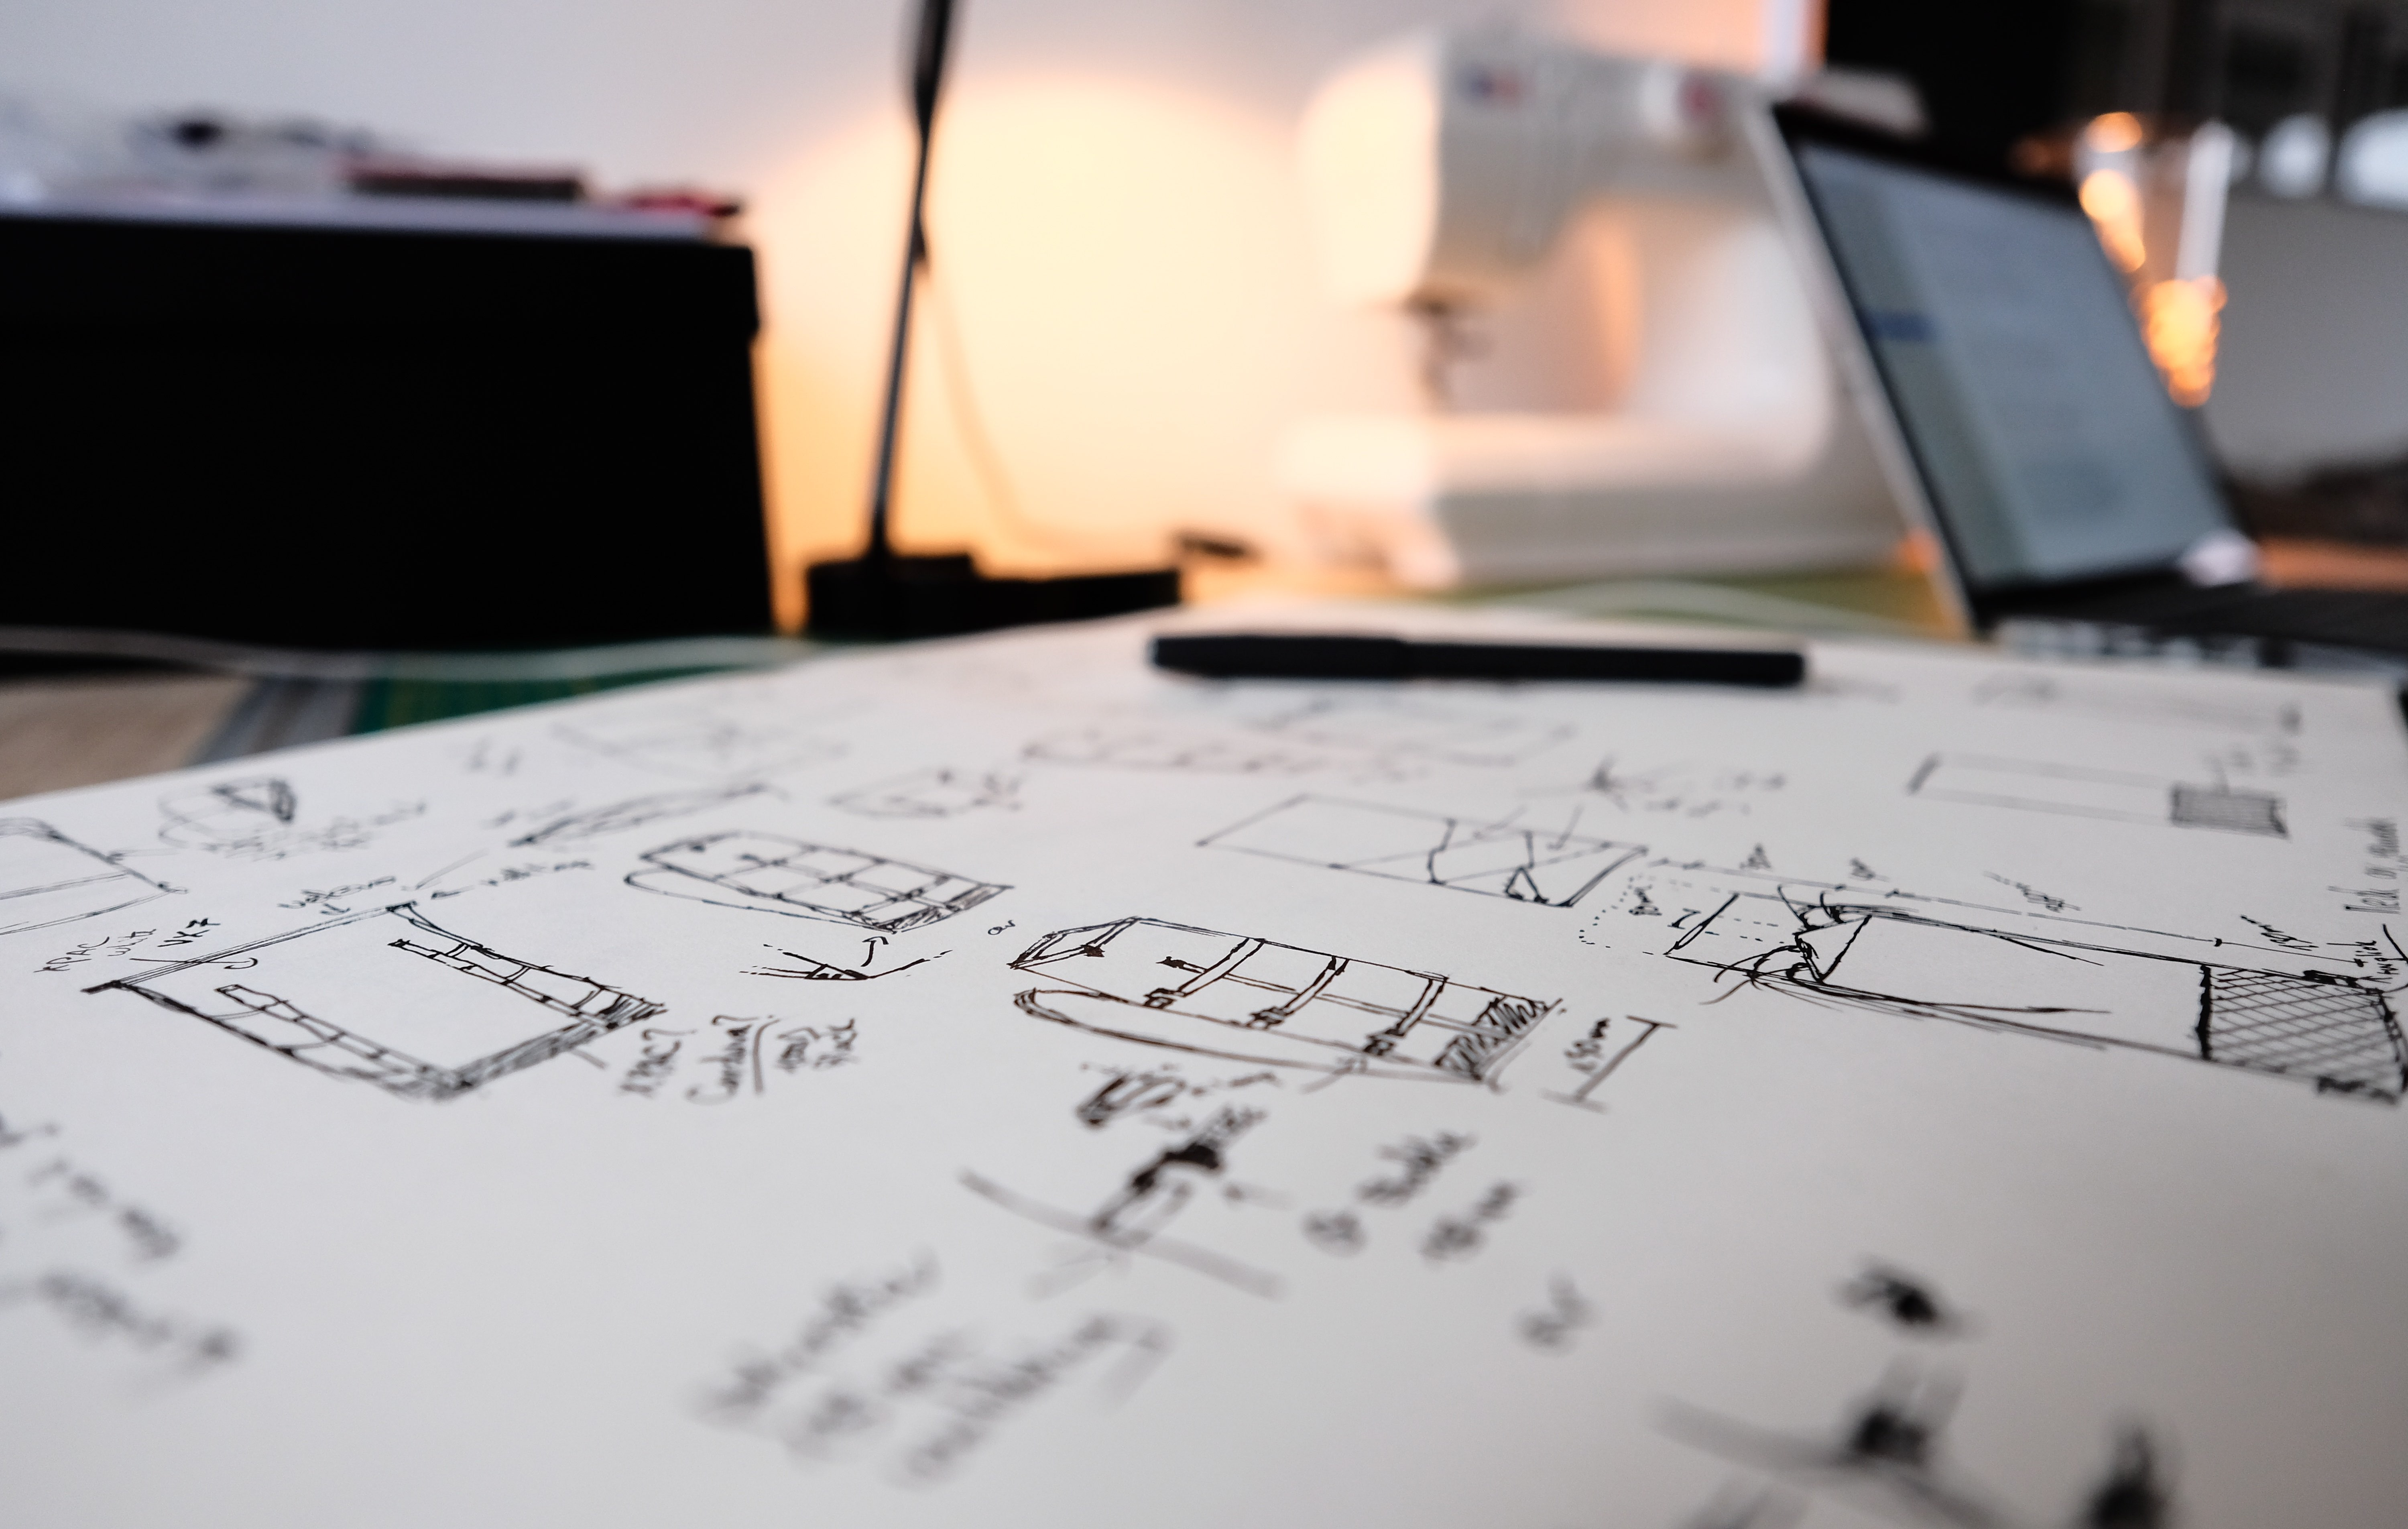
\includegraphics[width=\textwidth]{media/images/workspace-1}
  \caption{My workspace when I cleaned it up}
  \label{img:workspace-1}
\end{figure}
